\chapter{モデルを使った研究の進め方}


\section{アヤメ(iris)に関する推論}
公開されているアヤメのデータを使って、研究の進め方について検討する。
このアヤメのデータでは$3$種(setosa,versicolor,virginica)のがく片の幅、がく片の長さ、花弁の幅、花弁の長さのデータが記録されている。
データサイズは、150で、種によって$50$ずつ記録されている。Pythonのライブラリsklearnから簡単にデータを呼び出せる。
\begin{lstlisting}
from sklearn import datasets
iris = datasets.load_iris()
\end{lstlisting}

\subsection{アヤメのがく弁の幅を予測するモデル}
ここでは、アヤメという植物が見つかったときどのようにモデルを構築するかを考える。
アヤメについてその種が3種類の分類が行われる前で、1種類であると考える。
%我々が得ているのは、アヤメという植物のがく片の幅のデータ$150$個である。

我々は、がく弁の幅を予測するモデルを構築したい。
この目的を達成できるかはわからないが、一手目に行うのは、データに適合するモデルを探索することである。
データをみると、ある点を対称に同じくらいの数のデータがあることがわかる。
このことから、正規モデルが候補にあげられる。
データから平均と分散を求めると、$\bar{X}=3.05,\sigma=0.434$であった。
このことから、最尤正規モデルを構築する$M_a=M(3.05,\sigma^2=0.434^2)$である。
最尤正規モデルがデータに適合しているかをみる。
このモデルの予想では、$\mu$より大きいまたは小さいデータの個数は半数程度である。
また、$\mu-\sigma \sim \mu+\sigma$の中にあるデータは$68\%$程度である。
表\ref{table:all_spael_width_table}がデータが予測にあっているかを示している。
どちらの指標も予想に合っている。
また、$>\mu$と$\mu<$となるデータの個数の比率も$1$に近い$1.24$であった。
これはモデルがデータに適合していることを示している。
\begin{table}[h]
    \caption{aa}
    \label{table:all_spael_width_table}
    \centering
    \begin{tabular}{lccccccc}
        %\toprule
        \hline
        {} &  $<\mu$ &  $>\mu$ &  Data Size &  $<\mu$ Rate &  $>\mu$ Rate &  $<\mu/>\mu$ & $\mu-\sigma\sim\mu+\sigma$\\
        %\midrule
        \hline
        All    &    83 &    67 &        150 &       0.55 &       0.45 &       1.24 & 0.673\\
        %\bottomrule
        \hline
    \end{tabular}
\end{table}

\begin{figure}
    \begin{center}
        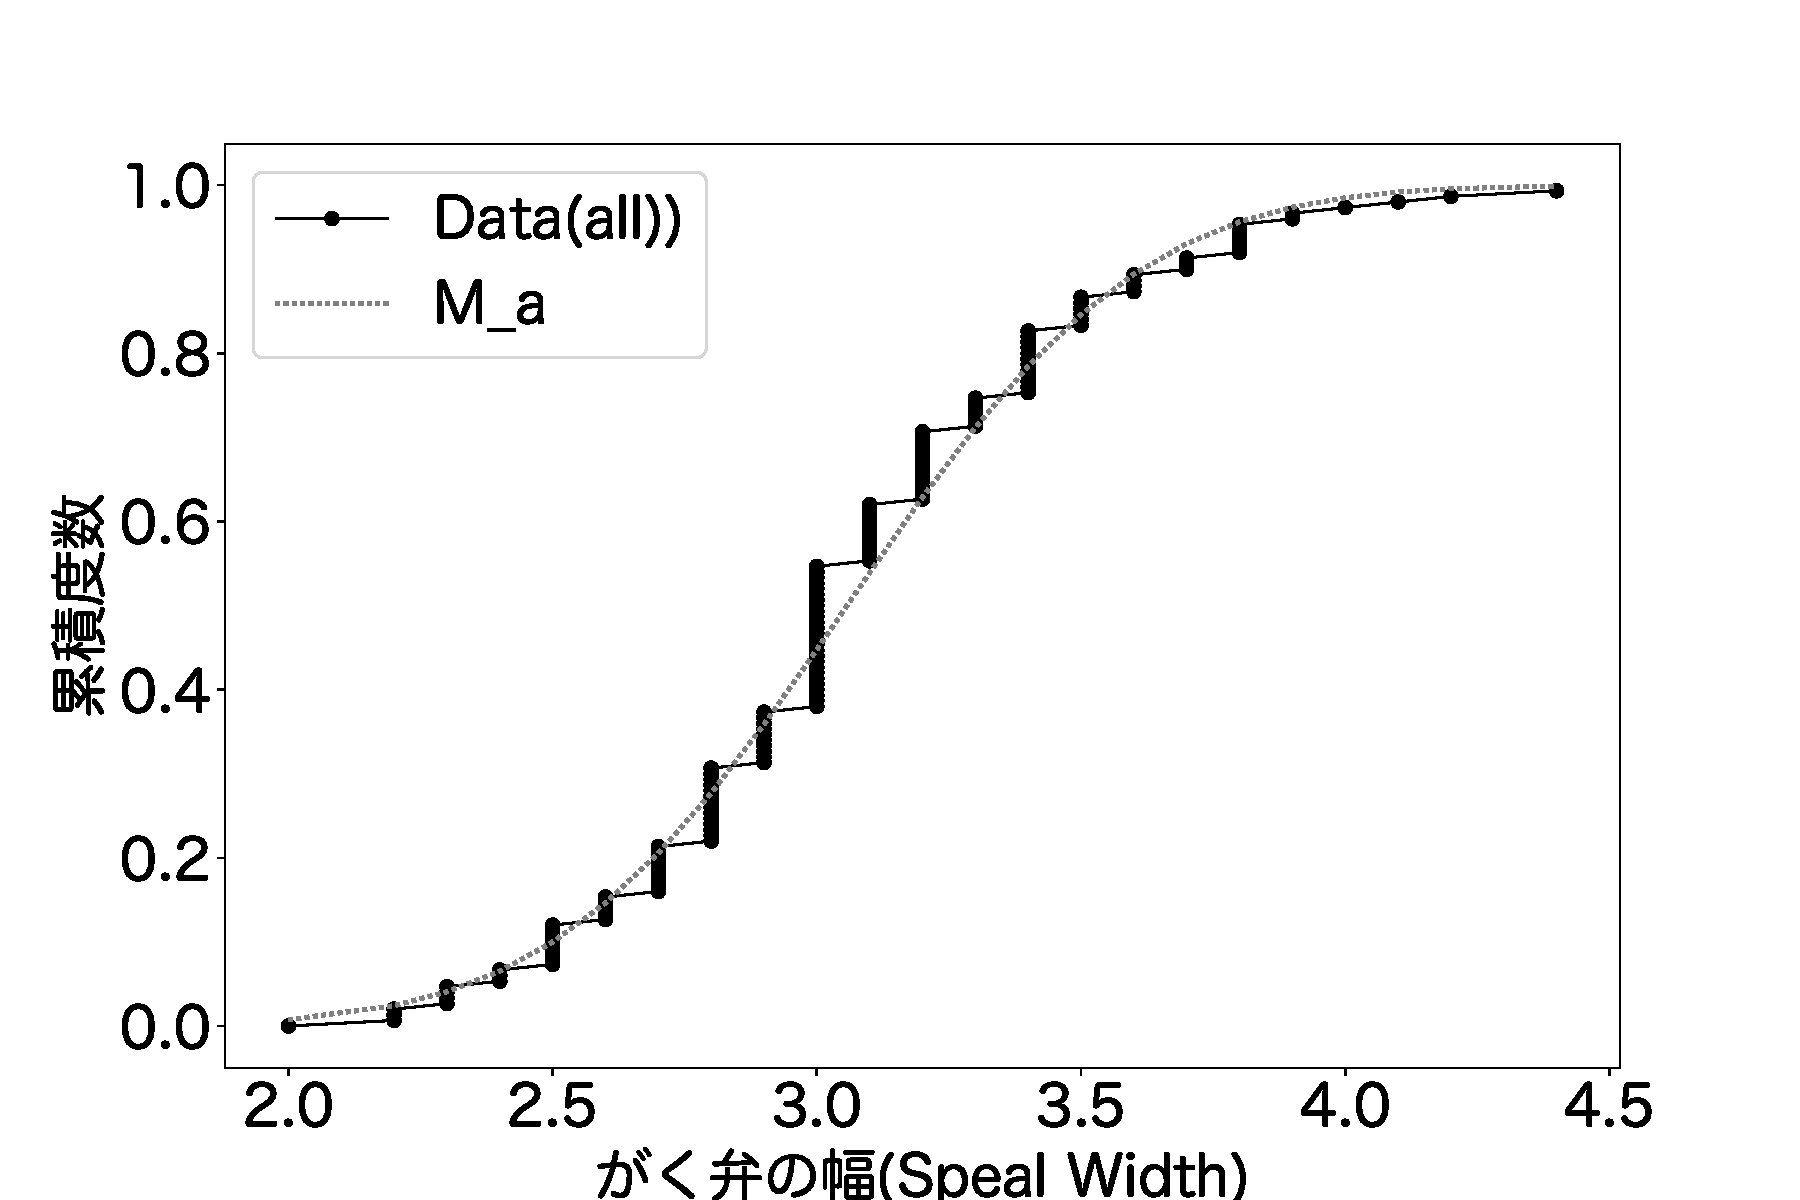
\includegraphics[width=15cm]{./image/15_/speal_width_all.pdf}
        \caption{データのがく弁の幅の累積度数(Data)と最尤モデルの累積度数$M_a$}
        \label{fig:all_speal_width_fig}
    \end{center}
\end{figure}

図\ref{fig:all_speal_width_fig}は、データの累積度数とモデルの累積度数を示している。
データとモデルの累積度数に関する予測がそれなりに一致していることがわかる。
このこともモデルがデータに適合していることを示唆している。

%アヤメについて統計モデルを使って予測する。
\subsection{アヤメの分類の細分化}
アヤメの分類を細分することになり、virginicaとそれ以外とすることになった。
これら二つのグループにおいて、がく弁の幅はこれまでに作ったモデル$M_a$により予測することができるだろうか。
新たにデータを取得し、モデルの予測とデータを比べることでモデル$M_a$の予測性能を測ることができる。
今回はデータを得るのが難しいので、もう一度同じデータを使い、モデルのデータに対する予測性能を測る\footnote{モデル構築に使ったデータを再び使うので、モデル$M_a$の予測の良さを測れていない}。
表\ref{table:speal_width_virig}がモデル$M_a$の予測に対する実際のデータの性質を示している。
virginicaとそれ以外はモデル$M_a$によって十分予測できていない。
モデル$M_a$の平均母数$\mu$より小さなものと大きなものの比が1より離れた値を取っている。
また、データの$68\%$が見つかるという予測をする区間には、$68\%$とはかけ離れた割合のデータが存在する。
図\ref{fig:virginica_speal_width_fig}には、モデル$M_a$とデータの累積度数を表示している。
モデル$M_a$の累積度数の上にデータの点がないことからも、モデルとデータが乖離していることが示唆される。
 

\begin{table}[h]
    \caption{アヤメ(virginicaとそれ以外)のがく弁の幅に関するデータの割合。モデル$M_a$の平均値を$\mu$としたとき、$\mu$より小さなデータの個数と割合($<\mu$、$<\mu$ Rate)。$\mu$より大きなデータの個数($>\mu$)と割合($>\mu$Rate)。$<\mu$と$>\mu$の割合。$\mu-\sigma\sim \mu+\sigma$の中にあるデータの個数($68\%$)と割合($68\%$Rate)。}
    \label{table:speal_width_virig}
    \centering
    \begin{tabular}{lrrrrrrrr}

        %\toprule
        \hline
        {} &  $<\mu$ &  $>\mu$ &  $<\mu$ Rate &  $>\mu$ Rate &  $<\mu/>\mu$ &  $68\%$ &  $68\%$Rate &  Data Size \\
        %\midrule
        \hline \hline
        virginica   &     8 &    42 &       0.16 &       0.84 &       0.19 &   27 &     0.54 &         50 \\
        others &    75 &    25 &       0.75 &       0.25 &       3.00 &   74 &     0.74 &        100 \\
        %All    &    83 &    67 &       0.55 &       0.45 &       1.24 &  101 &     0.67 &        150 \\
        %\bottomrule
        \hline
    \end{tabular}
\end{table}
    
\begin{figure}
    \begin{center}
        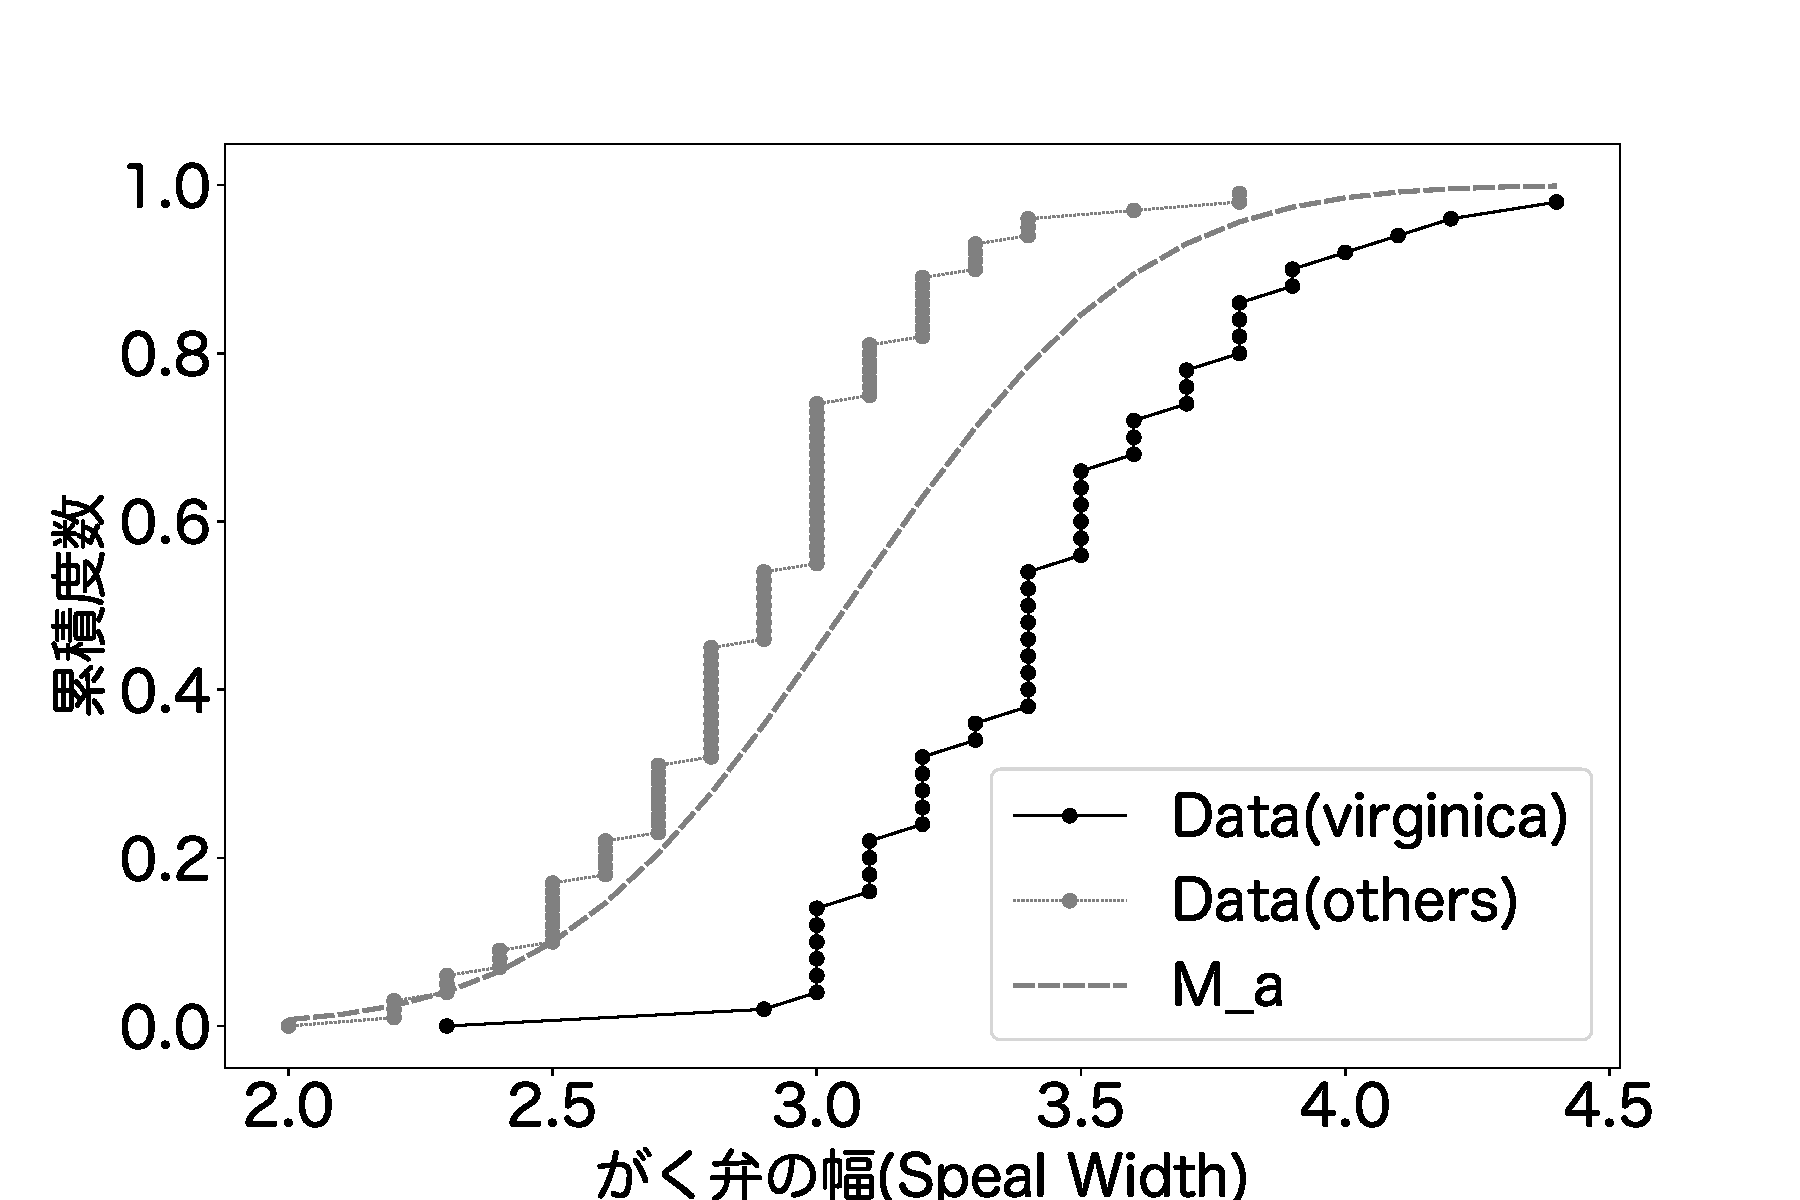
\includegraphics[width=15cm]{./image/15_/speal_width_viri.pdf}
        \caption{データのがく弁の幅の累積度数(Data)と最尤モデルの累積度数$M_a$}
        \label{fig:virginica_speal_width_fig}
    \end{center}
\end{figure}

モデル$M_a=M(\mu=3.05,\sigma^2=0.434^2)$における統計検定量も利用する。
次のことがわかっている。
\begin{equation*}
    Z = \frac{\sqrt{N}(\mu-\bar{x})}{\sigma} \sim N(0,1)
\end{equation*}
統計検定量$Z$を計算した結果が表\ref{table:speal_width_Z}である。
$Z$の絶対値は、$2$より大きくモデルとデータが乖離していることがわかる。

\begin{table}
    \caption{統計検定量$Z$}
    \label{table:speal_width_Z}
    \centering
    \begin{tabular}{lccc}
        \hline
        {} &   $\bar{x} $ &  $\sigma$  &     Z \\
        \hline \hline
        virginica &  3.43 &  0.38 & -6.03 \\
        others    &  2.87 &  0.33 &  4.27 \\
        $M_a$ & 3.05 & 0.434 & - \\
        \hline
    \end{tabular}
\end{table}

これらのことから、モデルの改訂をした方が良いことが示唆される。

以上のことは論文においては、統計統計量より偏った値が得られる確率($p$値)または$p<0.05$が報告される。
すでに議論した通り、$p$値だけでモデルとデータの乖離を検証すると、モデルの予測性能が過度に低いと判定されることがある。さまざまな指標を元にモデルの予測性能を測るべきである。

\subsection{新たなモデルの構築}
virginicaとothersに適合するモデルをそれぞれ構築する。
累積分布はどちらも正規分布的になっている。$M_a$を構築するときと同じようにそれぞれの平均と分散を求め(表\ref{table:speal_width_Z}の通りである)、データが平均に対して対称に分布していること、$\mu-\sigma\sim\mu+\sigma$の間にあるデータが$68\%$程度であるかを確かめる。

\begin{table}
    \caption{新たなモデル$M_v,M_o$による予測とデータの適合具合}
    \label{table:speal_width_replace_model}
    \begin{tabular}{lrrrrrrr}
        %\toprule
        \hline
        {} &  $<\mu$ &  $>\mu$ &  $<\mu$Rate &  $>\mu$Rate &  $<\mu/>\mu$  &  $68\%$Rate &  Sample Size \\
        %\midrule
        \hline \hline
        0 &   28 &   22 &     0.56 &     0.44 &      1.27 &     0.72 &           50 \\
        1 &   46 &   54 &     0.46 &     0.54 &      0.85 &     0.72 &          100 \\
        %\bottomrule
        \hline
    \end{tabular}
\end{table}   

表\ref{table:speal_width_replace_model}には、新たなモデル$M_v$および$M_o$の予測とデータの適合具合を示している。
どの指標もモデルの予想と一致しており、モデルがデータと適合していることを示唆している。

\begin{figure}
    \begin{center}
        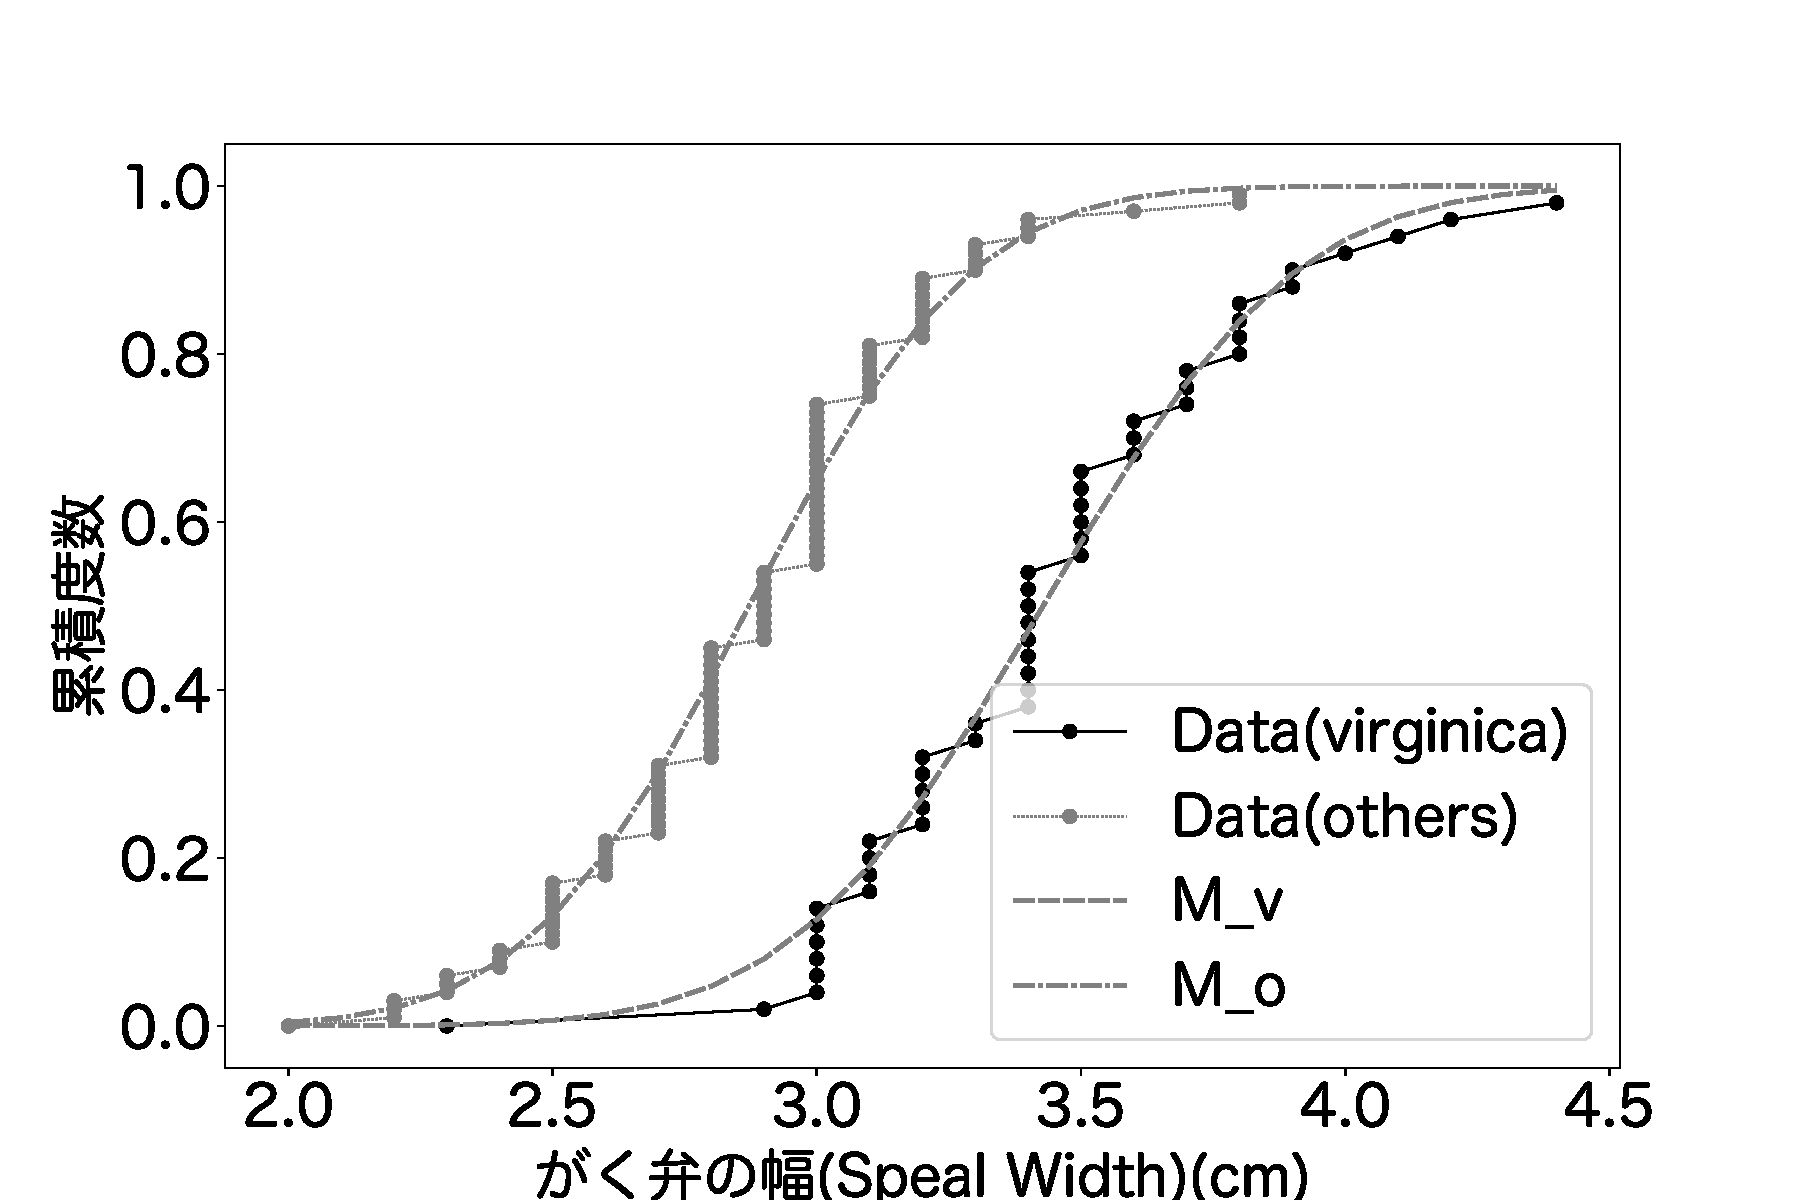
\includegraphics[width=15cm]{./image/15_/speal_width_viri_model.pdf}
        \caption{データのがく弁の幅の累積度数(Data)と最尤モデルの累積度数$M_v,M_o$}
        \label{fig:speal_width_viri_model}
    \end{center}
\end{figure}

図\ref{fig:speal_width_viri_model}はモデルの累積度数とデータの適合具合を示している。
それぞれのモデルがそれぞれデータをよく予測していることがわかる

\subsection{更なる細分化}
アヤメのothersについても細分化することになったsetosa,versicolorである。これらについて予測モデル$M_v$は良い予測をするかを調べ、予測できないと判断したのなら、モデルを構築し直すことになる。
